% Using Free and Open Source Solutions in Geospatial Science Education
% This work by Vaclav Petras is licensed under
% a Creative Commons Attribution-ShareAlike 4.0 International License.

\documentclass[xcolor={dvipsnames,usenames},beamer,aspectratio=1610]{beamer}
% ,handout,notes=show
% ,aspectratio=169

\makeatletter
\def\beamer@framenotesbegin{% at beginning of slide
  \gdef\beamer@noteitems{}%
  \gdef\beamer@notes{{}}% used to be totally empty.
}
\makeatother

\usepackage{textcomp}
\usepackage[utf8]{inputenc}
\usepackage[american]{babel}
\usepackage{graphicx}
\usepackage{url}

\usepackage{tikz}
\usetikzlibrary{arrows,shapes,spy,calc}

\tikzstyle{every picture}+=[remember picture]
\tikzstyle{na} = [baseline=-.5ex]

% frames have to be fragile
\newif\ifnotes
% \input{tmpnotessettings}
% \notestrue


\ifnotes
\setbeamertemplate{note page}[plain]
% \setbeamertemplate{note page}[compress]
\setbeamerfont{note page}{size=\large}
% \setbeameroption{show only notes}
\setbeameroption{show notes}
\usepackage{pgfpages}
\pgfpagesuselayout{2 on 1}[a4paper,border shrink=5mm]%
\else
%\setbeameroption{hide notes}
\fi
%\notesfalse

\usepackage[absolute,overlay]{textpos}

\usepackage{listings}


% \usetheme{Warsaw}
\usetheme{Madrid}
% \usetheme{Frankfurt}
% \useoutertheme{infolines}
\usecolortheme[named=MidnightBlue]{structure}
% \usecolortheme[named=PineGreen]{structure}
\setbeamertemplate{navigation symbols}{}

\setbeamertemplate{itemize items}[default]
\setbeamertemplate{enumerate items}[default]
% \useinnertheme{rectangles}
\setbeamertemplate{blocks}[default]


%%%%%%%%%%%%%%%%%%%%%%%%%%%%%%%%%%%%%%%%%%%%%%%%%%%%%%%%%%%%%%%%%%%%
%%%%%%%%%%%%%%%%%%%%%%%%%%%%%%%%%%%%%%%%%%%%%%%%%%%%%%%%%%%%%%%%%%%%

% \newcommand{\n}[1]{$^{\color{gray}{\mbox{\tiny#1}}}$}
\newcommand{\n}[1]{$^{\textcolor{gray}{\mbox{\tiny{#1}}}}$}

%%%%%%%%%%%%%%%%%%%%%%%%%%%%%%%%%%%%%%%%%%%%%%%%%%%%%%%%%%%%%%%%%%%%%%%%%%%%%%%
\newcommand{\gmodule}[1]{\href{http://grass.osgeo.org/grass71/manuals/#1.html}{\emph{#1}}}
\newcommand{\asixmodule}[1]{\emph{#1}}
\newcommand{\asevenmodule}[1]{\emph{#1}}
\newcommand{\module}[1]{\emph{#1}}
\newcommand{\grasslink}{\href{http://grass.osgeo.org/}{GRASS GIS}}

%%%%%%%%%%%%%%%%%%%%%%%%%%%%%%%%%%%%%%%%%%%%%%%%%%%%%%%%%%%%%%%%%%%%
%%%%%%%%%%%%%%%%%%%%%%%%%%%%%%%%%%%%%%%%%%%%%%%%%%%%%%%%%%%%%%%%%%%%

\title%[Processing of point clouds]
{Efficient processing of dense UAV point clouds}
\subtitle{Class project presentation}
%\pdforstring{}{}

\author[Vaclav Petras]
{Vaclav Petras (Vashek)%\n{1}\\
%{\scriptsize
%Anna Petrasova\n{1},
%\mbox{
%Helena Mitasova\n{1}
%}
%}
}

\institute[NC State University]
{%
%$^1$%
North Carolina State University, Center for Geospatial Analytics \\
\bigskip

\includegraphics[width=0.3\textwidth]{logos/ncstate}
}

\date[UAV/lidar data analytics course]{December 1, 2015\\
  \href{http://ncsu-osgeorel.github.io/uav-lidar-analytics-course}{GIS595/MEA792:
UAV/lidar data analytics course}}

\setbeamercovered{transparent}

\hypersetup{%
 pdfauthor={Vaclav Petras},%
 pdfsubject={UAV/lidar data analytics course project presentation},%
 pdfkeywords={UAV} {UAS} {point clouds} {lidar}
   {v.in.lidar} {r.in.lidar} {v.decimate} {v.out.lidar} {libLAS}
   {geospatial modeling} {GRASS GIS}
   {free software} {open source} {open science}
}

\usepackage{tipa}
\newcommand{\pron}[2]{#1 [#2]}


\newcommand{\beginbackup}{
  \newcounter{framenumbervorappendix}
  \setcounter{framenumbervorappendix}{\value{framenumber}}
}
\newcommand{\backupend}{
  \addtocounter{framenumbervorappendix}{-\value{framenumber}}
  \addtocounter{framenumber}{\value{framenumbervorappendix}}
}


%%%%%%%%%%%%%%%%%%%%%%%%%%%%%%%%%%%%%%%%%%%%%%%%%%%%%%%%%%%%%%%%%%%%
% when images are placed in these directories, we don't have to specify the directory
% just the filename
\graphicspath{{img/}{figures/}{images/}}


%%%%%%%%%%%%%%%%%%%%%%%%%%%%%%%%%%%%%%%%%%%%%%%%%%%%%%%%%%%%%%%%%%%%
%%%%%%%%%%%%%%%%%%%%%%%%%%%%%%%%%%%%%%%%%%%%%%%%%%%%%%%%%%%%%%%%%%%%
%%%%%%%%%%%%%%%%%%%%%%%%%%%%%%%%%%%%%%%%%%%%%%%%%%%%%%%%%%%%%%%%%%%%
%%%%%%%%%%%%%%%%%%%%%%%%%%%%%%%%%%%%%%%%%%%%%%%%%%%%%%%%%%%%%%%%%%%%
\begin{document}

\newcommand{\logowidth}{1.0em}
\newcommand{\logospace}{\hspace{0.2em}}
\newcommand{\includecclogo}[1]{\includegraphics[width=\logowidth]{./images/logos/#1}}

%%%%%%%%%%%%%%%%%%%%%%%%%%%%%%%%%%%%%%%%%%%%%%%%%%%%%%%%%%%%%%%%%%%%
\frame{
\titlepage
\begin{center}
\vspace{-3ex}
\href{http://creativecommons.org/licenses/by-sa/4.0/}{
\includecclogo{cc}
\logospace
\includecclogo{by}
\logospace
\includecclogo{sa}
}
\end{center}
}


%%%%%%%%%%%%%%%%%%%%%%%%%%%%%%%%%%%%%%%%%%%%%%%%%%%%%%%%%%%%%%%%%%%%%
\begin{frame}{}

\begin{block}{Questions}
 \begin{itemize}
  \item How many points are really necessary to create a detailed DEM?
  \item Which method of point decimation preserve more information?
 \end{itemize}
\end{block}

\begin{block}{Implementation}
 \begin{itemize}
  \item Open source implementation for further review and improvement.
  \item Methods implemented in GRASS GIS so that they can be used by a broad audience.
 \end{itemize}
\end{block}

\end{frame}


%%%%%%%%%%%%%%%%%%%%%%%%%%%%%%%%%%%%%%%%%%%%%%%%%%%%%%%%%%%%%%%%%%%%%
\begin{frame}{Count-based decimation influence on interpolated elevation}

\newcommand{\imgsize}{0.23\textwidth}


\centering
\begin{tikzpicture}[spy using outlines={circle,yellow,magnification=2,size=2.5cm, connect spies}]%
\node {%
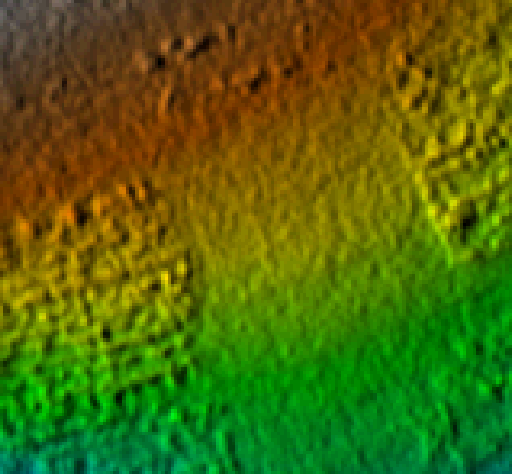
\includegraphics[width=\imgsize]{uav_all_shaded_elevation}%
~%
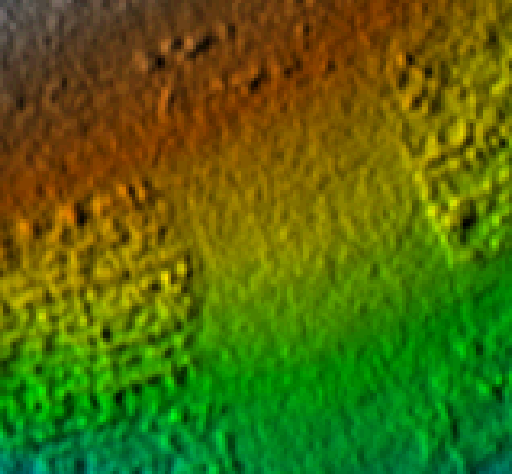
\includegraphics[width=\imgsize]{uav_skip_5_shaded_elevation}%
~%
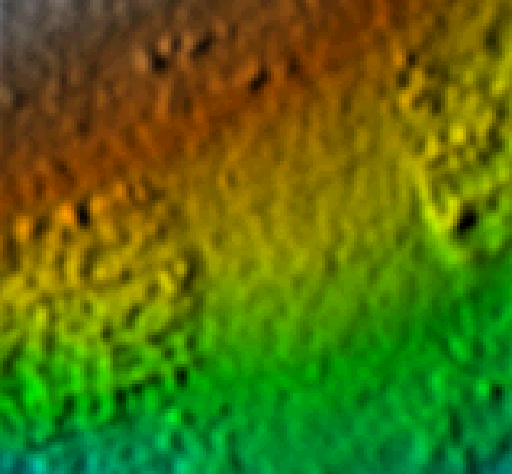
\includegraphics[width=\imgsize]{uav_preserve_20_shaded_elevation}%
~%
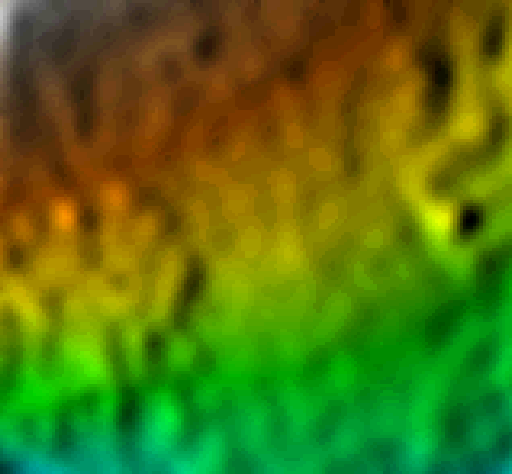
\includegraphics[width=\imgsize]{uav_preserve_100_shaded_elevation}%
};%
\spy on (-5.9,-0.5) in node [left] at (-3,2.25);%
\spy on (-2.3,-0.5) in node [left] at (0.6,2.25);%
\spy on (1.3,-0.5) in node [left] at (4.2,2.25);%
\end{tikzpicture}%

\newcommand{\captionfont}{\small}%
\makebox[\imgsize][c]{\captionfont all}%
~%
\makebox[\imgsize][c]{\captionfont skip=5}%
~%
\makebox[\imgsize][c]{\captionfont preserve=20}%
~%
\makebox[\imgsize][c]{\captionfont preserve=100}%

\makebox[\imgsize][c]{\captionfont 0 \%}%
~%
\makebox[\imgsize][c]{\captionfont 20 \%}%
~%
\makebox[\imgsize][c]{\captionfont 90 \%}%
~%
\makebox[\imgsize][c]{\captionfont 99 \%}%

\smallskip

\begin{flushleft}

\texttt{
g.region
%n=219454.8
%s=219410.1
%w=636937.5
%e=636985.8
nsres=0.3
ewres=0.3
rows=149
cols=161
\textit{(cells=23989)}
}

\texttt{
v.surf.rst
%input=..
%elevation=...
...
%aspect=...
%slope=...
npmin=120
tension=20
smooth=2
segmax=40
}

\end{flushleft}

\end{frame}


%%%%%%%%%%%%%%%%%%%%%%%%%%%%%%%%%%%%%%%%%%%%%%%%%%%%%%%%%%%%%%%%%%%%%
\begin{frame}{Count-based decimation influence on local relief model}

\newcommand{\imgsize}{0.23\textwidth}

\centering
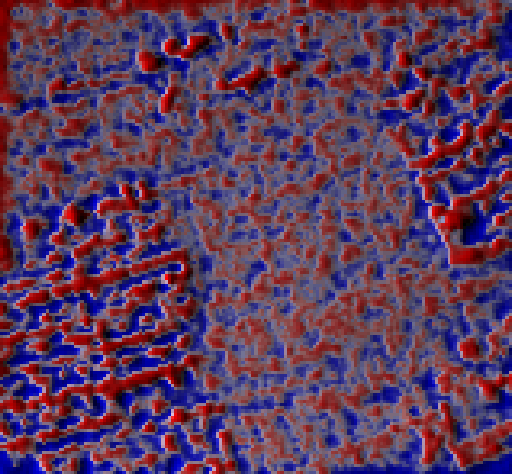
\includegraphics[width=\imgsize]{uav_all_lrm_shaded}%
~%
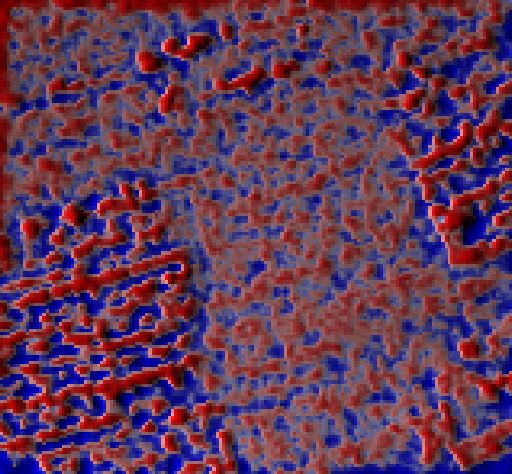
\includegraphics[width=\imgsize]{uav_skip_5_lrm_shaded}%
~%
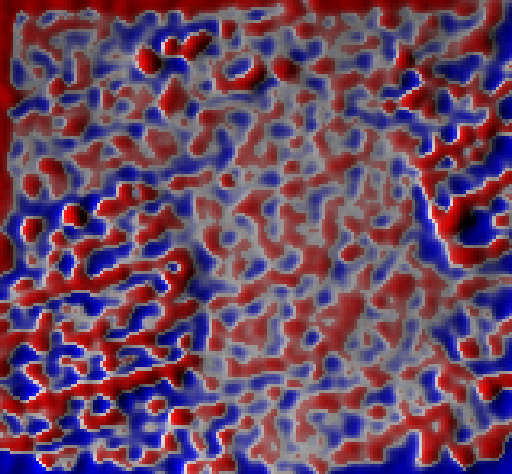
\includegraphics[width=\imgsize]{uav_preserve_20_lrm_shaded}%
~%
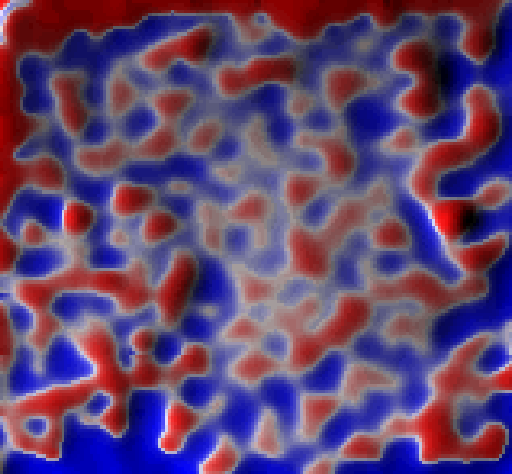
\includegraphics[width=\imgsize]{uav_preserve_100_lrm_shaded}%

\newcommand{\captionfont}{\small}%
\makebox[\imgsize][c]{\captionfont all}%
~%
\makebox[\imgsize][c]{\captionfont skip=5}%
~%
\makebox[\imgsize][c]{\captionfont preserve=20}%
~%
\makebox[\imgsize][c]{\captionfont preserve=100}%

\makebox[\imgsize][c]{\captionfont 0 \%}%
~%
\makebox[\imgsize][c]{\captionfont 20 \%}%
~%
\makebox[\imgsize][c]{\captionfont 90 \%}%
~%
\makebox[\imgsize][c]{\captionfont 99 \%}%

\bigskip

\begin{flushleft}

\texttt{
r.local.relief
input=...
output=...
shaded\_output=...
neighborhood=11
}

% r.covar ...

\end{flushleft}

\end{frame}


%%%%%%%%%%%%%%%%%%%%%%%%%%%%%%%%%%%%%%%%%%%%%%%%%%%%%%%%%%%%%%%%%%%%%
\begin{frame}{Progressiveness of count-based decimation}

\begin{center}
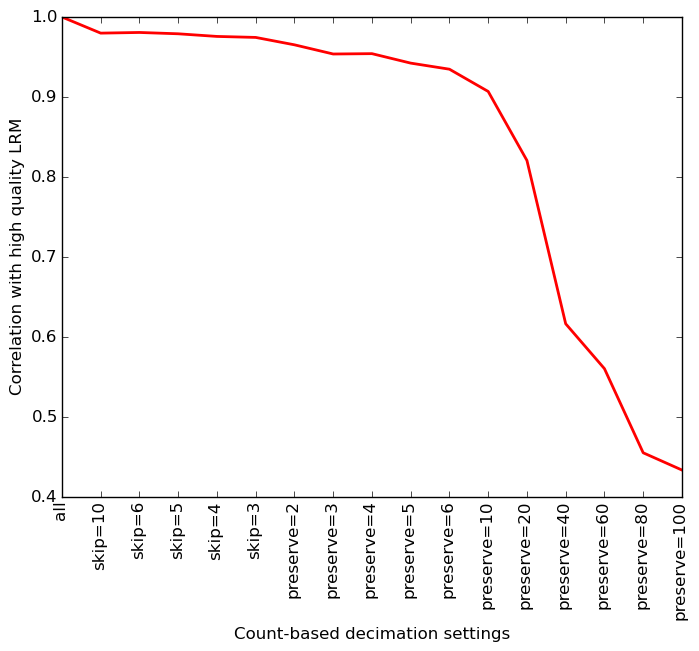
\includegraphics[height=0.8\textheight]{lrm_count}
\end{center}

\end{frame}


%%%%%%%%%%%%%%%%%%%%%%%%%%%%%%%%%%%%%%%%%%%%%%%%%%%%%%%%%%%%%%%%%%%%%
\begin{frame}{Influence of grid-based decimation resolution}

\newcommand{\imgsize}{0.23\textwidth}

\centering
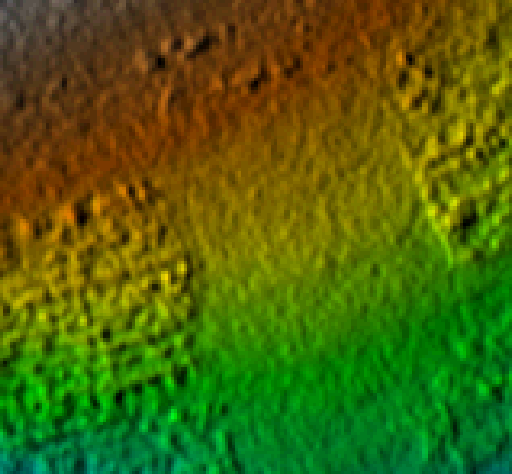
\includegraphics[width=\imgsize]{uav_grid_points_res_0_1_shaded_elevation}%
~%
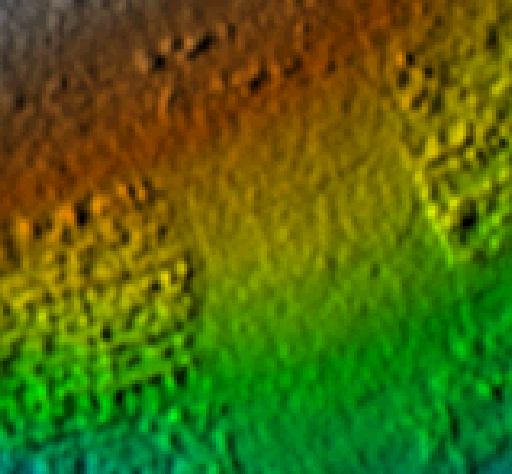
\includegraphics[width=\imgsize]{uav_grid_points_res_0_3_shaded_elevation}%
~%
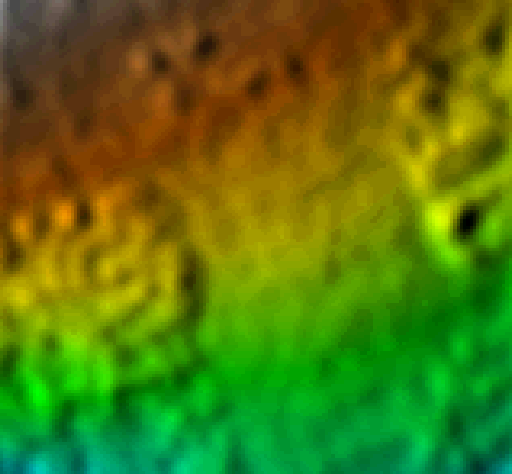
\includegraphics[width=\imgsize]{uav_grid_points_res_0_9_shaded_elevation}%
~%
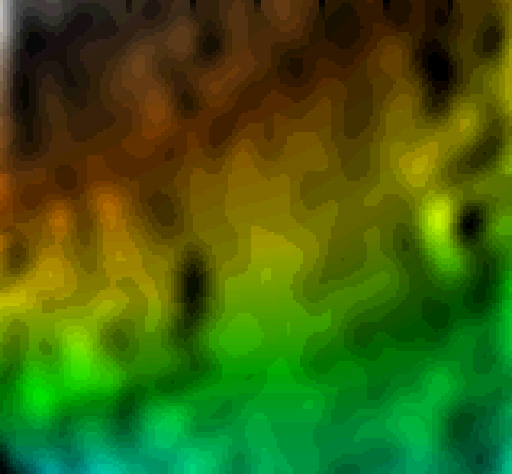
\includegraphics[width=\imgsize]{uav_grid_points_res_1_5_shaded_elevation}%

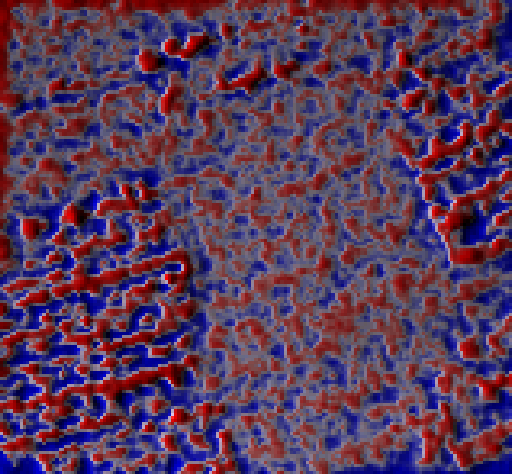
\includegraphics[width=\imgsize]{uav_grid_points_res_0_1_lrm_shaded}%
~%
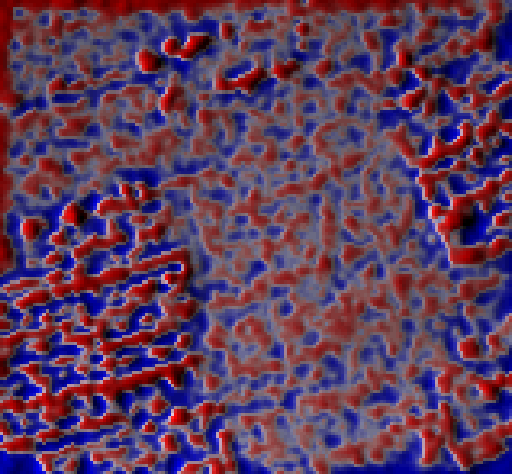
\includegraphics[width=\imgsize]{uav_grid_points_res_0_3_lrm_shaded}%
~%
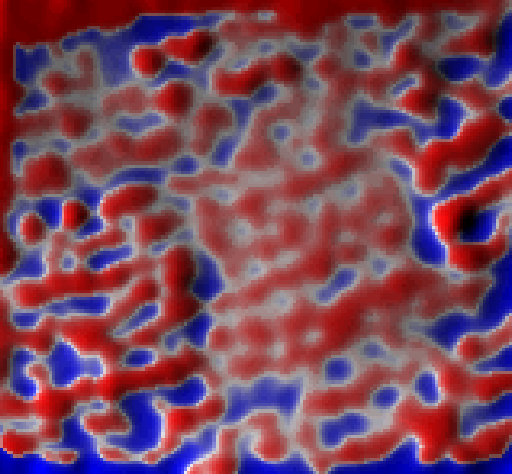
\includegraphics[width=\imgsize]{uav_grid_points_res_0_9_lrm_shaded}%
~%
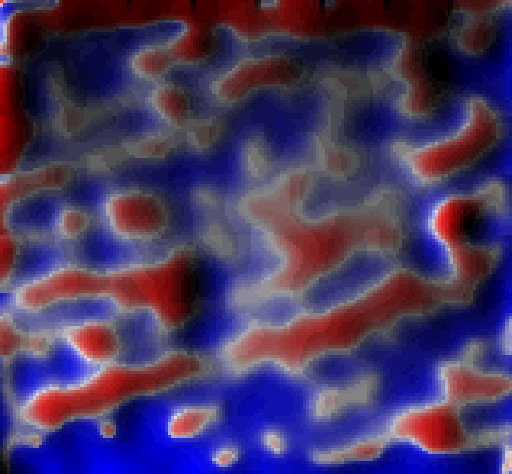
\includegraphics[width=\imgsize]{uav_grid_points_res_1_5_lrm_shaded}%

\newcommand{\captionfont}{\small}%
\makebox[\imgsize][c]{\captionfont resolution=0.1}%
~%
\makebox[\imgsize][c]{\captionfont resolution=0.3}%
~%
\makebox[\imgsize][c]{\captionfont resolution=0.9}%
~%
\makebox[\imgsize][c]{\captionfont resolution=1.5}%

\makebox[\imgsize][c]{\captionfont 0 \%}%
~%
\makebox[\imgsize][c]{\captionfont 81 \%}%
~%
\makebox[\imgsize][c]{\captionfont 98 \%}%
~%
\makebox[\imgsize][c]{\captionfont 99 \%}%

\end{frame}


%%%%%%%%%%%%%%%%%%%%%%%%%%%%%%%%%%%%%%%%%%%%%%%%%%%%%%%%%%%%%%%%%%%%%
\begin{frame}{Resolution of grid-based decimation}

\begin{center}
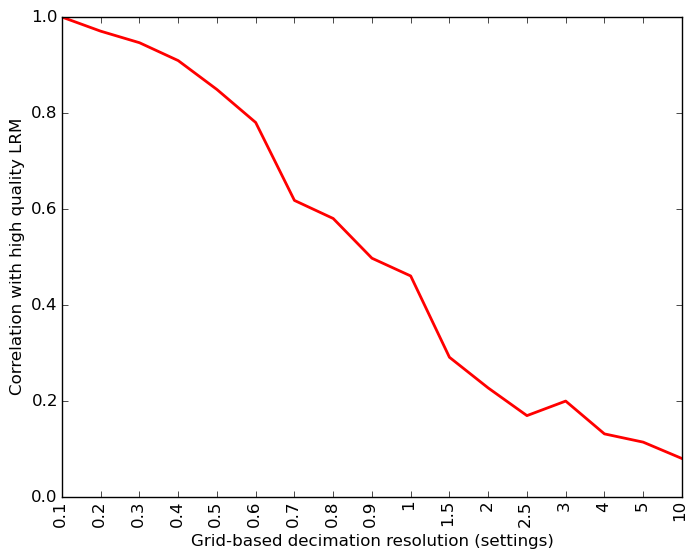
\includegraphics[height=0.8\textheight]{lrm_grid}
\end{center}

\end{frame}


%%%%%%%%%%%%%%%%%%%%%%%%%%%%%%%%%%%%%%%%%%%%%%%%%%%%%%%%%%%%%%%%%%%%%
\begin{frame}{Comparison of count-based and grid-based decimation}

\begin{center}
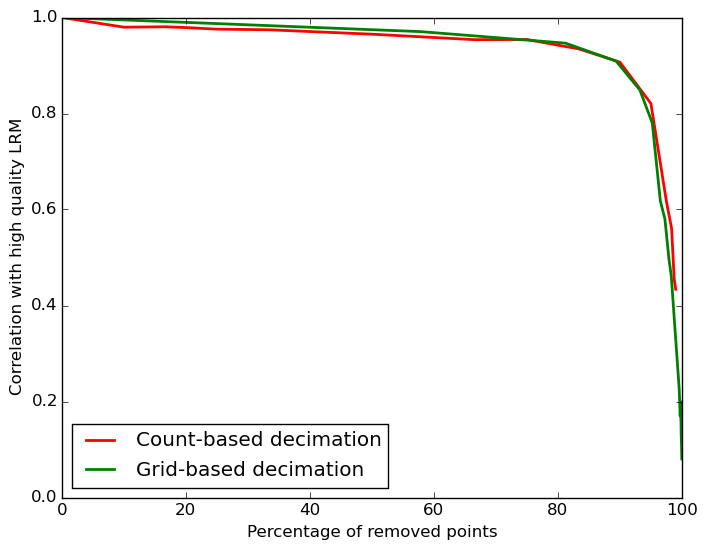
\includegraphics[height=0.8\textheight]{lrm_comparison_grid_count}
\end{center}

\end{frame}


%%%%%%%%%%%%%%%%%%%%%%%%%%%%%%%%%%%%%%%%%%%%%%%%%%%%%%%%%%%%%%%%%%%%%
%\begin{frame}{Merge point clouds as vector maps}

%v.patch: flags to work without topology and with z

%v.lidar.mcc: do not build topology in 7.1
%This is enabled by the change in v.patch.
%This makes it little bit faster.

%\end{frame}


%%%%%%%%%%%%%%%%%%%%%%%%%%%%%%%%%%%%%%%%%%%%%%%%%%%%%%%%%%%%%%%%%%%%%
\begin{frame}{Crop the point cloud by polygon}

\gmodule{v.in.lidar} -- limit the import to selected areas (2D)

\bigskip
\bigskip

\centering
\begin{minipage}{0.96\textwidth}
%
\newcommand{\imgsize}{0.23\textwidth}
\includegraphics<1->[width=\imgsize]{features/areas}%
~%
\only<-1>{\rule{\imgsize}{0pt}}%
\includegraphics<2->[width=\imgsize]{features/selected_1}%
~%
\only<-2>{\rule{\imgsize}{0pt}}%
\includegraphics<3->[width=\imgsize]{features/selected_2}%
~%
\only<-3>{\rule{\imgsize}{0pt}}%
\includegraphics<4->[width=\imgsize]{features/merged}%

\newcommand{\captionfont}{\scriptsize\tt}%
% using phantom to vertically stretch to have space for p
\makebox[\imgsize][c]{\captionfont areas\vphantom{patch}}%
~%
\only<-1>{\rule{\imgsize}{0pt}}%
\only<2->{\makebox[\imgsize][c]{\captionfont v.in.lidar mask=}}
~%
\only<-2>{\rule{\imgsize}{0pt}}%
\only<3->{\makebox[\imgsize][c]{\captionfont v.in.lidar -i mask=}}%
~%
\only<-3>{\rule{\imgsize}{0pt}}%
\only<4->{\makebox[\imgsize][c]{\captionfont v.patch -nz}}%
%
\end{minipage}

\end{frame}

%%%%%%%%%%%%%%%%%%%%%%%%%%%%%%%%%%%%%%%%%%%%%%%%%%%%%%%%%%%%%%%%%%%%%
\begin{frame}{Count-based decimation}

\gmodule{v.in.lidar} -- count-based decimation during import

\begin{center}
\begin{minipage}{0.96\textwidth}
%
\newcommand{\imgsize}{0.23\textwidth}
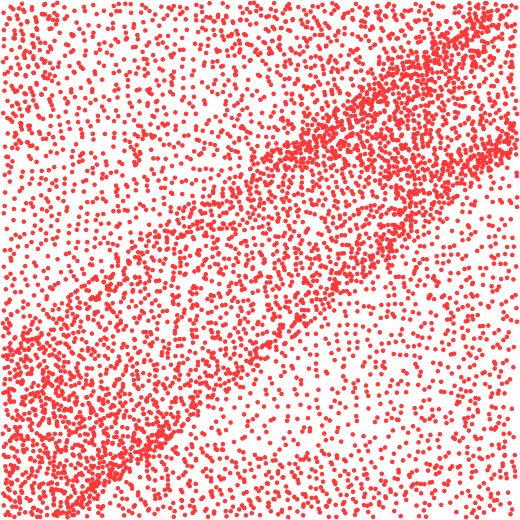
\includegraphics[width=\imgsize]{features/full}%
~%
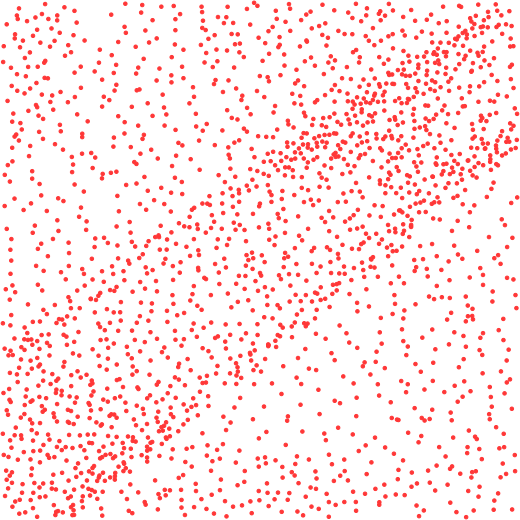
\includegraphics[width=\imgsize]{features/preserve}%
~%
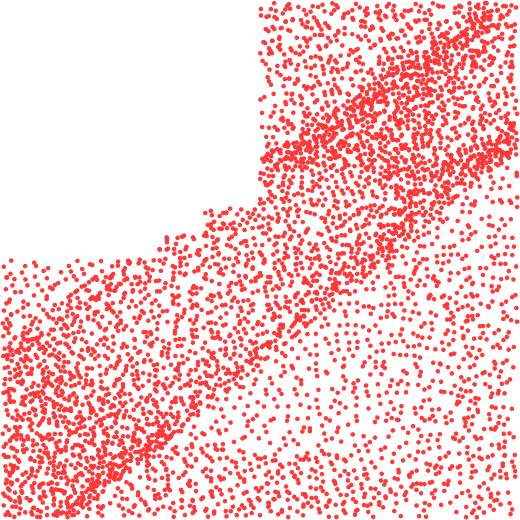
\includegraphics[width=\imgsize]{features/offset}%
~%
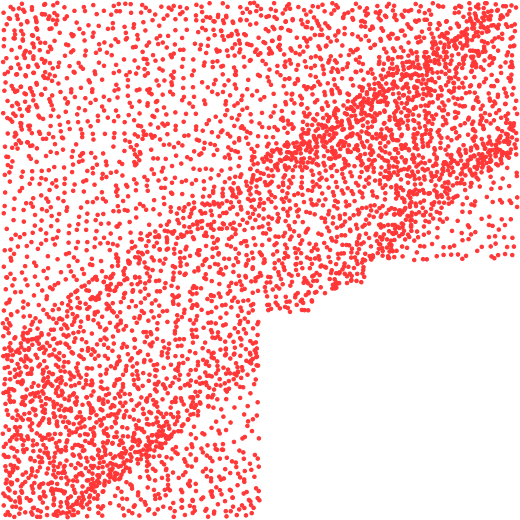
\includegraphics[width=\imgsize]{features/limit}%

\newcommand{\captionfont}{\small}%
% using phantom to vertically stretch to have space for p
\makebox[\imgsize][c]{\captionfont full}%
~%
\makebox[\imgsize][c]{\captionfont preserve/skip}
~%
\makebox[\imgsize][c]{\captionfont offset}%
~%
\makebox[\imgsize][c]{\captionfont limit}%
%
\end{minipage}
\end{center}

\gmodule{v.decimate} -- point cloud decimation of vector maps
(also supports grid-based decimation with preserving point properties)

\end{frame}


%%%%%%%%%%%%%%%%%%%%%%%%%%%%%%%%%%%%%%%%%%%%%%%%%%%%%%%%%%%%%%%%%%%%%
\begin{frame}{Store return and class information as category}

\gmodule{v.in.lidar} can store return or class information as category

{\small using layers and categories for something else than ID and class}
% Storing information as categories of vector points

% fastest: -cb
% potentially -r + decimations

\begin{center}
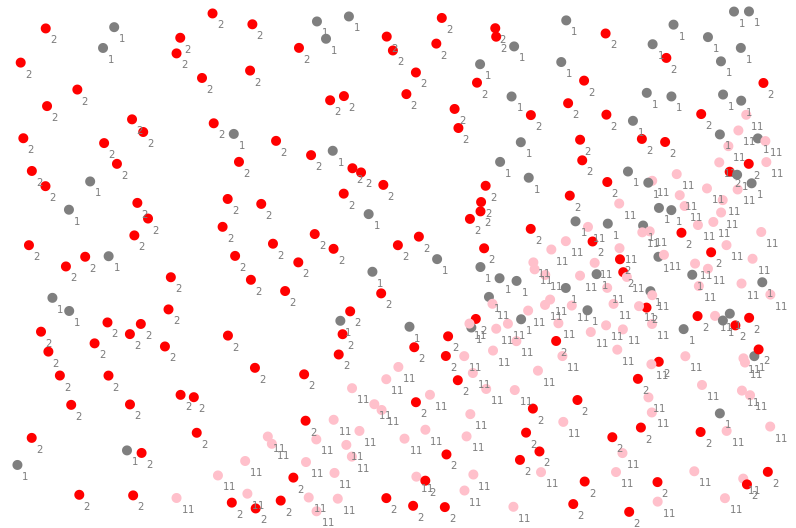
\includegraphics[height=0.6\textheight]{images/features/class_as_cat}
\end{center}

Also: read coordinates only -- speed improvement (\texttt{-c} flag)

\end{frame}


%%%%%%%%%%%%%%%%%%%%%%%%%%%%%%%%%%%%%%%%%%%%%%%%%%%%%%%%%%%%%%%%%%%%%
\begin{frame}{Binning of points from multiple LAS files}

\gmodule{r.in.lidar} -- read multiple LAS files in one run

\bigskip
\small

The original workflow

\smallskip

\texttt{ r.in.lidar input=tile\_01.las output=tile\_01}\\
\texttt{ r.in.lidar input=tile\_02.las output=tile\_02}\\
\texttt{ ...}\\
\texttt{ r.patch input=tile\_01,tile\_02,... output=elevation}\\

\smallskip

is replaced by

\smallskip

\alert{
\texttt{ r.in.lidar file=tile\_list.txt output=elevation}\\
}

\smallskip

where \texttt{tile\_list.txt} is

\smallskip

\texttt{ tile\_01.las}\\
\texttt{ tile\_02.las}\\
\texttt{ ...}\\

\end{frame}

%%%%%%%%%%%%%%%%%%%%%%%%%%%%%%%%%%%%%%%%%%%%%%%%%%%%%%%%%%%%%%%%%%%%%
%\begin{frame}{Filter points using range for Z coordinates}

%remove prominent outliers during import with \gmodule{v.in.lidar}

%\centering
%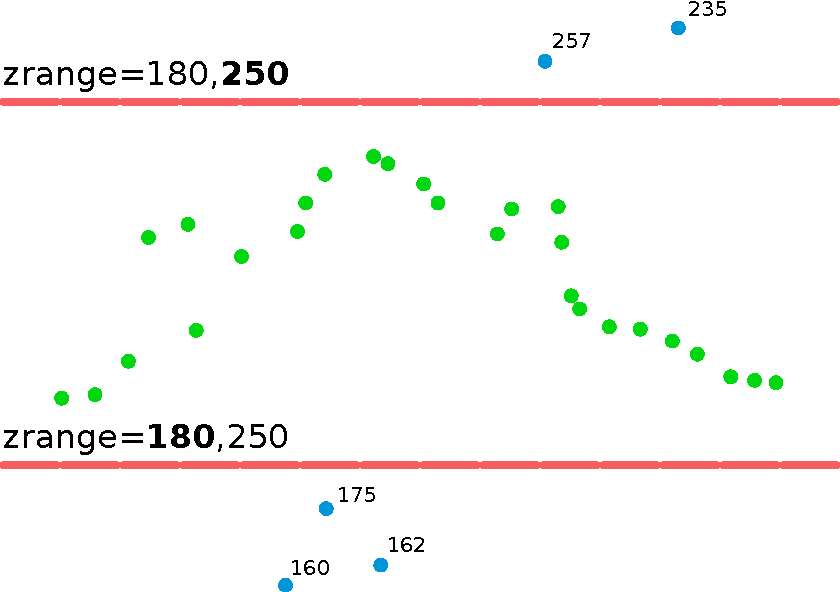
\includegraphics[height=0.7\textheight]{images/features/zrange}

%\end{frame}

%%%%%%%%%%%%%%%%%%%%%%%%%%%%%%%%%%%%%%%%%%%%%%%%%%%%%%%%%%%%%%%%%%%%%
\begin{frame}{Compute height above a given raster during binning}

\gmodule{r.in.lidar} -- derive height above ground of features

\begin{center}
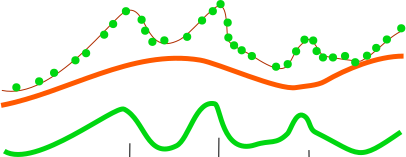
\includegraphics[height=0.5\textheight]{images/features/base_raster}
\end{center}

The resolutions of binning and ground raster can differ, so different
statistics can be computed during binning.

\end{frame}


%%%%%%%%%%%%%%%%%%%%%%%%%%%%%%%%%%%%%%%%%%%%%%%%%%%%%%%%%%%%%%%%%%%%%
\begin{frame}{Export vector points from GRASS GIS as LAS}

\gmodule{v.out.lidar} -- export points in a vector map as lidar points

\begin{itemize}
\item visualization (plas.io, CloudCompare)
\item further processing (PDAL, libLAS, CloudCompare, \ldots)
\item testing workflows with generated data
\end{itemize}

\begin{center}
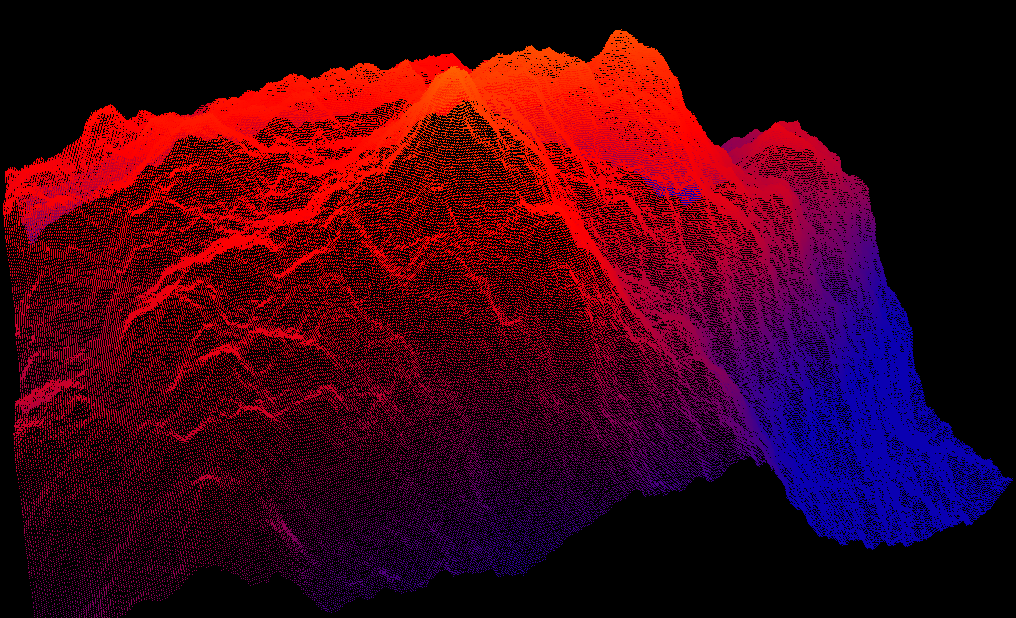
\includegraphics[height=0.5\textheight]{images/features/fractals_plasio}

\gmodule{r.surf.fractal} output in \href{http://plas.io}{plas.io}
\end{center}

% g.region rows=1669 cols=2515 cells=4197535
% r.surf.fractal out=test
% r.to.vect -z t=p in=test out=test -b
% v.out.lidar in=test out=test.las

\end{frame}


%%%%%%%%%%%%%%%%%%%%%%%%%%%%%%%%%%%%%%%%%%%%%%%%%%%%%%%%%%%%%%%%%%%%%
%\begin{frame}{Future work and work in progress}

%\begin{itemize}
%\item show large point clouds in Map Display (2D) -- \module{d.points}
%\item colorize the points according to a raster -- \module{v.colorize}
%\item binning from a vector map -- \module{v.binning}, \module{r.binning}
%\item binning to a 3D raster -- \module{v.binning}, \module{r3.binning}, \module{r3.in.lidar}
%\item general support for color stored as category
    %-- \module{v.colors}, \module{d.vect}, \module{v.colorize}
%\item use PDAL as backend for import and export
    %-- \module{v.in.pdal}, \module{v.in.points}, \module{v.in.lidar}
%\item provide access to selected PDAL analyses
    %-- \module{v.in.pdal}, \module{v.pdal}
%\end{itemize}

%\end{frame}


%%%%%%%%%%%%%%%%%%%%%%%%%%%%%%%%%%%%%%%%%%%%%%%%%%%%%%%%%%%%%%%%%%%%%
\begin{frame}{}

% logo at the bottom can be moved down
\vspace*{0.05\textheight}

\begin{block}{Summary}
 \begin{itemize}
  \item count-based and grid-based decimation perform the same on a \emph{given} point cloud
  \item analysis needed for every dataset \textrightarrow{} need for tool to create a report
  \item improvements needed for the project integrated into GRASS GIS
 \end{itemize}
\end{block}

\bigskip

\centering
\href{https://grass.osgeo.org/download/}{%
Get GRASS GIS 7.1 development version at\\
\texttt{grass.osgeo.org/download}%
}

\smallskip


\includegraphics[height=0.25\textheight]{logos/grass_gis}

% this is for logo without text
%\vspace*{-1.5ex}
%\Large
%\textbf{GRASS} GIS

\end{frame}

\end{document}
